\documentclass[11pt]{article}

%TODO
\usepackage{xcolor}
\newcommand\myworries[1]{\textcolor{red}{#1}}
%%


\usepackage{report}
\usepackage{caption}
\usepackage{float}
\usepackage[utf8]{inputenc} % allow utf-8 input
\usepackage[italian]{babel}
\usepackage[T1]{fontenc}    % use 8-bit T1 fonts
\usepackage[colorlinks=true, linkcolor=black, citecolor=blue, urlcolor=blue]{hyperref}       % hyperlinks
\usepackage{url}            % simple URL typesetting
\usepackage{booktabs}       % professional-quality tables
\usepackage{amsfonts}       % blackboard math symbols
\usepackage{nicefrac}       % compact symbols for 1/2, etc.
\usepackage{microtype}      % microtypography
\usepackage{lipsum}		% Can be removed after putting your text content
\usepackage{graphicx}
\usepackage{natbib}
\usepackage{doi}
\setcitestyle{aysep={,}}

% tree structure
\usepackage{forest}
%%%%%%%%%


%%%%%%%%%%%%%% CODE

\usepackage{listings}
\usepackage{color} %red, green, blue, yellow, cyan, magenta, black, white
\definecolor{mygreen}{RGB}{28,172,0} % color values Red, Green, Blue
\definecolor{mylilas}{RGB}{170,55,241}

\lstset{language=Matlab,%
    %basicstyle=\color{red},
    breaklines=true,%
    morekeywords={matlab2tikz},
    keywordstyle=\color{blue},%
    morekeywords=[2]{1}, keywordstyle=[2]{\color{black}},
    identifierstyle=\color{black},%
    stringstyle=\color{mylilas},
    commentstyle=\color{mygreen},%
    showstringspaces=false,%without this there will be a symbol in the places where there is a space
    numbers=left,%
    numberstyle={\tiny \color{black}},% size of the numbers
    numbersep=9pt, % this defines how far the numbers are from the text
    emph=[1]{for,end,break},emphstyle=[1]\color{red}, %some words to emphasise
    %emph=[2]{word1,word2}, emphstyle=[2]{style},    
}

%----------------------------------------------------------------------------------------
%	PYTHON CODE THEMPLATE
%----------------------------------------------------------------------------------------
\usepackage{listings}
\usepackage{xcolor}

\definecolor{codegreen}{rgb}{0,0.6,0}
\definecolor{codegray}{rgb}{0.5,0.5,0.5}
\definecolor{codepurple}{rgb}{0.58,0,0.82}
\definecolor{backcolour}{rgb}{0.95,0.95,0.92}

\lstset{language=Matlab,%
     % backgroundcolor=\color{backcolour},
    commentstyle=\color{codegreen},
    keywordstyle=\color{magenta},
    numberstyle=\tiny\color{codegray},
    stringstyle=\color{codepurple},
    basicstyle=\ttfamily\footnotesize,
    breakatwhitespace=false,
    breaklines=true,
    captionpos=b,
    keepspaces=true,
    numbers=left,
    numbersep=5pt,
    showspaces=false,
    showstringspaces=false,
    showtabs=false,
    aboveskip=6mm,
    belowskip=6mm,
    tabsize=2   
}
%%%%%%%%%%%%%%

\title{Cholesky Analysis}

\author{
  \Large\textbf{Mario Avolio}\\
  \texttt{880995}
  \and
  \Large\textbf{Simone Benitozzi}\\
  \texttt{889407}
}

% Uncomment to remove the date
\date{\today}

% Uncomment to override  the `A preprint' in the header
\renewcommand{\headeright}{Cholesky Analysis - Metodi del calcolo Scientifico}
\renewcommand{\undertitle}{Metodi del calcolo Scientifico}
\renewcommand{\shorttitle}{}

%%% Add PDF metadata to help others organize their library
%%% Once the PDF is generated, you can check the metadata with
%%% $ pdfinfo template.pdf
% \hypersetup{
% pdftitle={A template for the arxiv style},
% pdfsubject={q-bio.NC, q-bio.QM},
% pdfauthor={David S.~Hippocampus, Elias D.~Striatum},
% pdfkeywords={First keyword, Second keyword, More},
% }

\begin{document}
\maketitle


\newpage
\thispagestyle{empty}
\tableofcontents

\newpage
\thispagestyle{empty}
\listoffigures


\newpage
\thispagestyle{empty}
\listoftables


\newpage
\thispagestyle{empty}
\setcounter{page}{1}

\section{Introduzione}
TODO: Introduzione


\section{Descrizione del dominio di riferimento e obiettivi della sperimentazione} 

\subsection{Risoluzione di Sistemi Lineari}

Il problema della risoluzione di sistemi lineari attraverso una computazione efficiente è tuttora aperto e al centro di progetti e obiettivi di ricerca.

Allo stato dell'arte attuale si definiscono due tipologie principali di metodologie per la loro risoluzione: i metodi diretti e i metodi iterativi.
I metodi diretti permettono di arrivare ad una soluzione in un numero finito di step e restituirebbero la soluzione esatta sotto l'assunzione di essere eseguiti su un'aritmetica con precisione infinita, cosa in realtà non possibile sui reali calcolatori.

La tecnica di base per una risoluzione di questo tipo è detta \textit{fattorizzazione LU} di una matrice A, che viene scomposta in una \textit{Lower triangular L} e una \textit{Upper triangular U}, con il risultato finale calcolato come segue:

\begin{equation} \label{eq1}
\begin{split}
Ax & = b \\
L(Ux) & = b; Ux = y \\
Ly & = b
\end{split}
\end{equation}

\begin{figure}[h!]
    \centering
    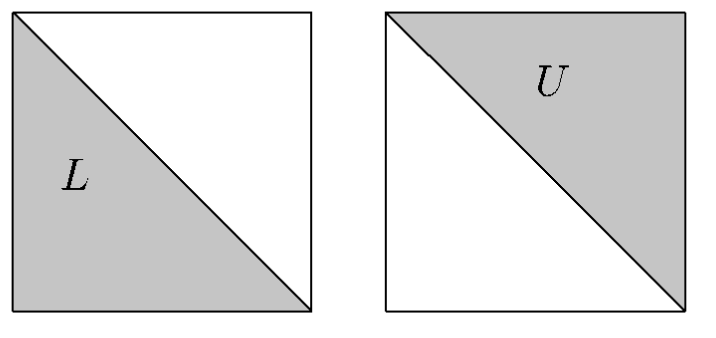
\includegraphics[width=0.5\textwidth]{figs/LU_decomposition.png}
    \caption{LU Decomposition for Direct Methods}
    \label{fig:LU_decomposition}
\end{figure}

Al contrario, i metodi iterativi non assicurano di terminare in un numero finito di step: a partire da un \textit{initial guess} formano iterazioni successive che convergono solo al limite della soluzione esatta. 
Per far sì che l'iterazioni termini, viene utilizzato un criterio di convergenza per specificare quando una soluzione approssima sufficientemente al risultato esatto. 

Anche in caso dell'utilizzo di un'aritmetica con precisione infinita, i metodi iterativi non restituirebbero comunque, in linea teorica, una soluzione esatta, ma il loro vantaggio è quello di essere computazionalmente più efficienti dei diretti, e pertanto più utilizzati nella pratica, sebbene abbiano la necessità di essere eseguiti su matrici che rispettino precise proprietà per essere certi della convergenza. Ad esempio, 2 tra i metodi iterativi più comuni, \textit{Jacobi} e \textit{Gauß-Seidel}, garantiscono la convergenza solo in caso di matrici a dominanza diagonale in input.

Nel presente elaborato viene analizzata la risoluzione di sistemi lineari mediante decomposizione di Cholesky, una particolare tipologia di metodo diretto che sfrutta la proprietà secondo cui, se la matrice \textit{A} è \textit{SDP} (simmetrica e definita positiva), è allora possibile riorganizzare la decomposizione in maniera tale che \textit{U} sia la trasposta di \textit{L}, pertanto \textit{A} possa essere riscritta come

\begin{equation} \label{eq1}
\begin{split}
Ax & = LL'
\end{split}
\end{equation}

\begin{figure}[h!]
    \centering
    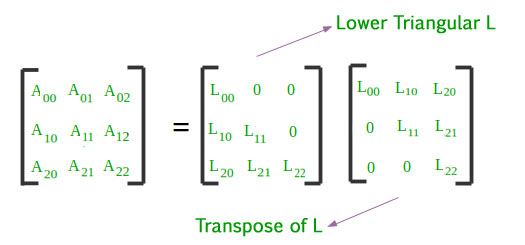
\includegraphics[width=0.75\textwidth]{figs/chol_decomposition.jpg}
    \caption{Basic visualization for Cholesky Decomposition}
    \label{fig:cholesky_decomposition}
\end{figure}

Se la matrice rispetta tale proprietà, allora è garantito che la sua decomposizione di Cholesky esista e sia unica, il che rende la risoluzione del sistema più efficiente e stabile rispetto ad una normale decomposizione \textit{LU}.

Come già visto precedentemente, sebbene si tratti di un metodo di risoluzione diretto, che pertanto dovrebbe, in linea teorica, restituire un risultato esatto a seguito di un numero finito di step, ciò non è garantito dal fatto di utilizzare dei calcolatori non provvisti di precisione aritmetica infinita.
È per questo che tra le analisi presentate in seguito, si terrà conto nella valutazione del miglior risultato, anche dell'errore relativo tra il risultato calcolato e quello atteso, auspicando comunque che esso si avvicini quanto più possibile all'epsilon di macchina, pari a
\[
  2.220446049250313*10^{-16}
\]

\subsection{Matrici Sparse}

Avendo a che fare con dati di dimensioni molto grandi, nelle analisi che seguono sono state utilizzate le matrici sparse: si tratta di matrici con la maggior parte dei valori pari a 0, che vengono memorizzate in maniera compatta, tenendo conto dei soli valori positivi.

\begin{figure}[h!]
    \centering
    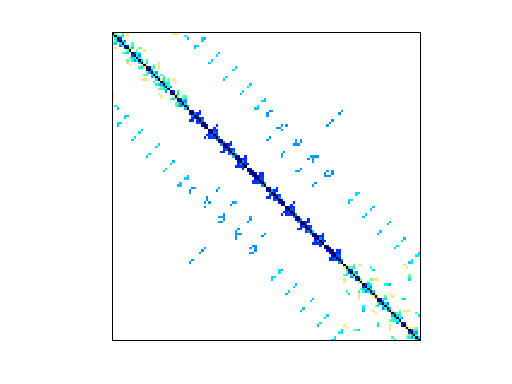
\includegraphics[width=0.5\textwidth]{figs/shallow_water1.png}
    \caption{Sparse matrix example}
    \label{fig:sparse_matrix_example}
\end{figure}

Questo modo di operare permette, oltre al fatto di risparmiare sapzio in memoria a seguito del cricamento della matrice stessa, anche una risoluzione più efficiente della decomposiiizione di Cholesky stessa.

La semplice decomposizione di Cholesky, applicata ad una matrice sparsa, ne causerebbe il \textit{fill-in}, a seguito della generazione di elementi diversi da 0. Ciò non accade in una particolare tipologia di matrici sparse, le matrici \textit{tridiagonali}, nelle quali gli elementi diversi da zero sono solo sulla diagonale principale e sulle due sottodiagonali.

Per trattare matrici sparse generali viene quindi effettuata una permutazione preliminare di righe e colonne in modo che l’algoritmo di Cholesky generi il minor numero possibile di elementi diversi da zero, per una risoluzione più efficiente e performante. 

\section{Scelte di Progettazione} % presentiamo il codice
Nella seguente sezione verranno trattati le principali scelte di progettazione atte all'analisi dei dati delle matrici e ai corrispettivi dati riscontrati dall'analisi. La figura \ref{fig:Progettazione} mostra i passi fondamentali eseguiti durante tutta la durata della sperimentazione:
\begin{enumerate}
    \item Esecuzione del metodo di Cholesky sulle singole Matrici al variare dell'OS e del linguaggio.
    \item Salvataggio dei dati riscontrati.
    \item Analisi dei dati.
\end{enumerate}
\begin{figure}[h!]
    \centering
    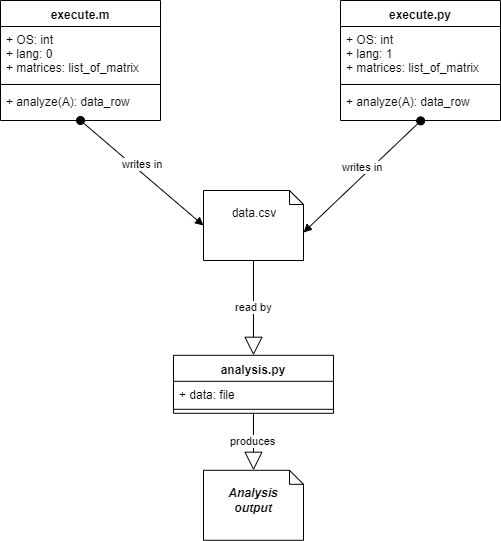
\includegraphics[width=0.5\textwidth]{figs/Structure Flowchart.png}
    \caption{Diagramma UML di progettazione}
    \label{fig:Progettazione}
\end{figure}
La seguente trattazione non ha il compito di definire in modo particolarmente tecnico tutta la fase di progettazione, bensi' si vuole soffermare su quegli aspetti ritenuti fondamentali per comprendere al meglio l'operato. Dalla figura \ref{fig:Progettazione} si possono notare anche molteplici altri aspetti:
\begin{enumerate}
    \item \textbf{Reperimento Dati:} sono stati utilizzati due script (\textit{execute.m} e \textit{execute.py}) per eseguire il metodo di Cholesky sulle varie matrici e per il reperimento dei corrispettivi dati. E' doveroso sottolineare che essi non hanno il compito di analizzare i dati da essi stessi prodotti. L'utilizzo di questa metodologia ha permesso una migliore divisione tra le componenti adibite al reperimento dei dati e quelle per la corrispettiva analisi. 
    Un approccio diverso sarebbe stato estramamente lento e poco preciso per una corretta e omogenea analisi.
    \item \textbf{Salvataggio Dati:} il salvataggio dei dati, riscontrati al punti precedente, avviene mediante un file \textit{data.csv} che verrà analizzato come se fosse un \textbf{dataset}.
    \item \textbf{Analisi dei Dati:} l'analisi dei dati è stata effettuata a posteriori rispetto al reperimento dati, in particolar modo dopo aver eseguito i due script sui sistemi operativi di interesse. Questa procedura ha permesso di analizzare i dati in maniera indipendente rispetto agli script atti al reperimento dei dati.
\end{enumerate}
Nelle prossime sezioni verranno trattati più in dettaglio i procedimenti sfruttati e le librerie utilizzate per lo scopo. Oltre a ciò verrà anche definita l'architettura sfruttata per l'esecuzione dei diversi Sistemi Operativi.
\subsection{L'utilizzo della Virtualizzazione}
Al fine di garantire una più pulita analisi dei dati si è optato per l'utilizzo della virtualizzazione dei sistemi Linux e Microsoft Windows, su cui si sono svolti i dovuti test. In particolare la scelta in ambiente linux si è rivolta sulla distribuzione \textbf{\href{https://lubuntu.me/}{Linux Lubuntu}}, mentre in ambiente Microfost Windows la scelta è ricaduta su \textbf{\href{https://www.microsoft.com/it-it/software-download/windows10}{Windows 10}}.
\paragraph{HyperVisor} Per favorire la miglior virtualizzazione possibile è stato necessario l'impiego dell'hypervisor~(\cite{itwiki:120906467}) che è il componente centrale e più importante di un sistema basato sulle macchine virtuali. Un computer sul quale venga eseguito un hypervisor che a sua volta controlla una o più macchine virtuali è detto macchina host, e ogni macchina virtuale è detta macchina guest. Il compito di un hypervisor è quello di presentare all'utente i sistemi operativi delle macchine guest e di gestire la loro esecuzione. Grazie ad un hypervisor, su una macchina host possono essere in esecuzione contemporaneamente diverse macchine guest, su ognuna delle quali può girare un sistema operativo diverso che ha il controllo sulle risorse hardware virtualizzate rese disponibili dall'hypervisor. La ragione per cui è stato scelto è inerente al fatto che questo tipo di virtualizzazione è diversa dalla virtualizzazione a livello di sistema operativo, dove tutte le istanze (dette anche container) devono essere eseguite in un unico kernel. \\
In particolar modo è opportuno sottolineare che per tale scopo è stato sfruttato \textbf{\href{https://docs.microsoft.com/it-it/virtualization/hyper-v-on-windows/about/}{Microsoft Hyper-V}}, ovvero un \textbf{HyperVisor di tipo 1} (\textit{native hypervisor}). Questa tipologia di virtualizzazione offre numerosi benefici rispetto agli \textbf{HyperVisor di tipo 2} (\textit{hosted hypervisor}). Sebbene in questa esposizione non si voglia entrare nel merito della questione, nella figura \ref{fig:HyperVisor} sono schematizzate le principali differenze tra i due sistemi di virtualizzazione. \\
è doveroso sottolineare che la virtualizzazione è stata eseguita sfruttando lo stesso \textit{hardware} per entrambi i sistemi operativi testati, in particolare ad ognuno di essi sono stati dedicati 6 core sulla CPU (\textit{Intel(R) Core(TM) i7-10710U CPU @ 1.10GHz 1.61 GHz}) e 8GB di RAM.
\begin{figure}[h!]
    \centering
    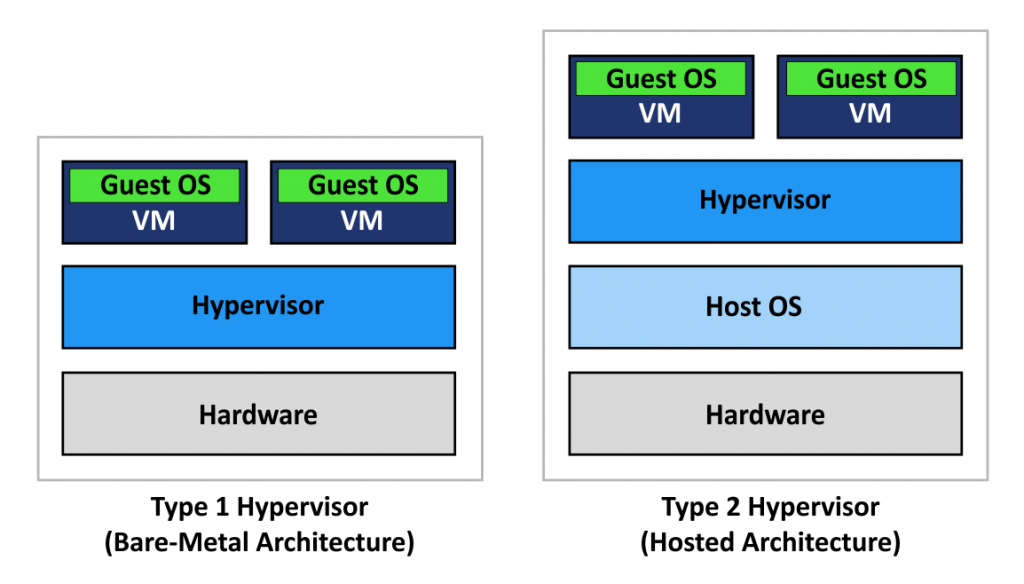
\includegraphics[width=1\textwidth]{figs/Type-1-and-type-2-hypervisor-1024x584.png}
    \caption{HyperVisor Types from \href{https://www.nakivo.com/blog/it/hyper-v-virtualbox-one-choose-infrastructure-2/}{www.nakivo.com}}
    \label{fig:HyperVisor}
\end{figure}

\section{Reperimento Dati}
Questa sezione ha il compito di introdurre più in dettaglio le strutture di progettazione (e i 
\subsubsection{Matlab}
\myworries{Come ho fatto il matlab? Puoi usare lstinputlisting per inserire codice matlab (già gestito da me nella sintassi di latex) }

\paragraph{Problemi Riscontrati e limitazioni}
\myworries{Problematiche riscontrate? Backslash funziona?}

\subsubsection{Python}
Per gestire al meglio la giusta separazione tra gli elementi del progetto si è deciso di sfruttare un particolare pattern strutturale definito dallo schema sottostante. Il modello, cattura il comportamento dell'applicazione in termini di dominio del problema e gestisce direttamente i dati, la logica e le regole del progetto. \\ Nella seguente trattazione, al fine di evitare panoramiche fuori focus, si vogliono sottolineare solo gli aspetti fondamentali utilizzati per il reperimento dei dati tramite l'esecuzione del metodo di Choleksy.


\begin{forest}
  for tree={
    font=\ttfamily,
    grow'=0,
    child anchor=west,
    parent anchor=south,
    anchor=west,
    calign=first,
    edge path={
      \noexpand\path [draw, \forestoption{edge}]
      (!u.south west) +(7.5pt,0) |- node[fill,inner sep=1.25pt] {} (.child anchor)\forestoption{edge label};
    },
    before typesetting nodes={
      if n=1
        {insert before={[,phantom]}}
        {}
    },
    fit=band,
    before computing xy={l=15pt},
  }
[PythonProject
   [src
      [Analyze
          [\_\_init\_\_.py]
          [analyze.py]
          [helper.py]
      ]
      [Model
          [\_\_init\_\_.py]
          [execute.py]
          [helper.py]
      ]
      [\_\_init\_\_.py]
      [costants.py]
    ]
]
\end{forest}\\

\paragraph{Lo script execute.py}
Lo script \textit{execute.py} svolge il ruolo primario dell'intero ecosistema python. Esso ha il compito di prendere in considerazione ogni matrice per poi analizzarla singolarmente mediante lo script \textit{analyze.py}. La figura \ref{fig:execute.py} ne mostra il funzionamento.
\begin{figure}[h!]
    \centering
    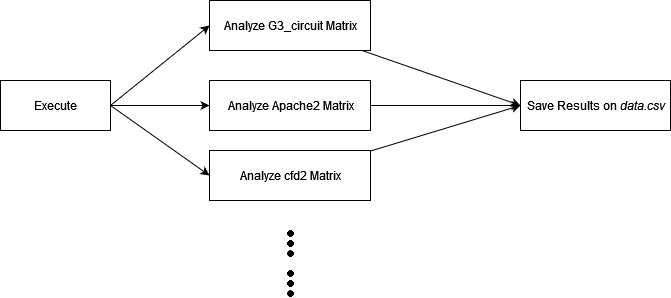
\includegraphics[width=0.7\textwidth]{figs/execute.drawio.png}
    \caption{Funzionamento dello script \textit{execute.py}}
    \label{fig:execute.py}
\end{figure}

\paragraph{Lo script analyze.py}
Il package \textbf{Analyze} si occupa principalmente di andare ad applicare ad una spefica matrice il metodo di \textbf{Cholesky}. Il codice \ref{AnalyzeClass} riporta l'implementazione della classe fondamentale situata nel file \textbf{analyze.py}.

\lstinputlisting[language=Python, caption= Analyze Class, label=AnalyzeClass]{CODE/Py/Analyze.py}

Come si può notare essa racchiude le parti fondamentali dell'operazione effettuata, in particolar modo si vuole sottolineare l'importanza della funzione \textbf{\_\_analyze(self, path)}. Essa prevede in input il \textit{path} dov'è situata la matrice da leggere. La funzione esegue i seguenti step:
\begin{enumerate}
    \item Lettura della Matrice
    \item Inizio dell'analisi sulla memoria occupata e sul tempo impiegato.
    \item Esecuzione del metodo di Cholesky
    \item Fine dell'analisi sulla memoria occupata e sul tempo impiegato.
    \item Calcolo dell'errore relativo rispetto alla soluzione fornita di default.
\end{enumerate}
Come si può facilmente notare dal codice \ref{AnalyzeClass}, si è predisposto il tutto per scrivere i risultati ottenuti in tabelle \textit{*.csv}, al fine di facilitarne l'analisi futura.

\paragraph{L'utilizzo di \textit{Scikit-Sparse}}
Python fornisce librerie di default per trattare matrici con il metodo di Cholesky, tra esse è doveroso nominare \textbf{Numpy}~(\cite{harris2020array}) e \textbf{SciPy}~(\cite{2020SciPy-NMeth}). Sfortunatamente queste librerie non foniscono un metodo diretto per analizzare \textbf{matrici sparse}, per cui la scelta è ricaduta su una libreria \textbf{open-source} chiamata \textbf{\href{https://scikit-sparse.readthedocs.io/en/latest/}{Scikit-Sparse}}. Essa si basa su \textit{SciPy.Sparse} ma, al contrario di quest'ultima, offre funzioni veloci ed efficienti per trattare matrici sparse con Cholesky. Il codice \ref{scikitsparsecholesky} mostra l'implementazione effettuata tramite l'utilizzo della libreria sopra indicata. Si noti che tale funzione viene richiamata dal metodo \_\_analyze(self, path) a riga \textit{21}.

\lstinputlisting[language=Python, caption= scikit\_sparse\_cholesky function, label=scikitsparsecholesky]{CODE/Py/scikitSparse.py}

\paragraph{Problemi Riscontrati e limitazioni}
La principale problematica, riscontrata durante la progettazione dell'ecosistema Python, ricade principalmente nella struttura della libreria utilizzata. Sfortunatamente la compilazione di \textit{Scikit-Sparse} non fornisce esito positivo in ambienti \textbf{Microsoft Windows}. I test sono stati effettuati mediante l'ausilio del package manager \href{https://pypi.org/project/pip/}{Pip} e \href{https://www.anaconda.com/products/distribution}{Anaconda}, ma nessuno ha dato buon fine. Per questo motivo si è ritenuto opportuno l'utilizzo della \textbf{WSL} (\textit{Windows Subsystem for Linux}) al fine di risolvere la problematica.
\subsection{Salvataggio Dati}
\myworries{Qui inseriamo il dataset prodotto}

\subsection{Analisi Dei Dati}
Nella seguente sottosezione verranno trattate le procedure di progettazione utilizzate durante l'analisi dei dati prodotti, in particolare le librerie utilizzate. In particolare i dati analizzati saranno quelli provenienti dai file \textit{*.csv}. Per far ciò è stato sfruttato \textit{JupyterBook} \cite{perez2011python} mediante il linguaggio Python. Di seguito viene proposta la struttura dell'intero progetto di analisi.\\
\begin{forest}
  for tree={
    font=\ttfamily,
    grow'=0,
    child anchor=west,
    parent anchor=south,
    anchor=west,
    calign=first,
    edge path={
      \noexpand\path [draw, \forestoption{edge}]
      (!u.south west) +(7.5pt,0) |- node[fill,inner sep=1.25pt] {} (.child anchor)\forestoption{edge label};
    },
    before typesetting nodes={
      if n=1
        {insert before={[,phantom]}}
        {}
    },
    fit=band,
    before computing xy={l=15pt},
  }
[PythonAnalysis
   [src
      [model
          [\_\_init\_\_.py]
          [additional\_analysis.ipynb]
          [backslash\_comparison.ipynb]
          [LanguageCompare.ipynb]
          [OSCompare.ipynb]
      ]
      [Resources
          [data.csv]
          [dataBackslash.csv]
      ]
    ]
]
\end{forest}\\
Si noti che l'analisi è stata volutamente strutturata in diverse sotto-analisi:
\begin{itemize}
    \item Analisi dei Linauggi
    \item Analisi degli OS
    \item Confronto metodo \textit{Chol} con \textit{Backslash} in Matlab
    \item Analisi aggiuntive e di interesse
\end{itemize}
\subsubsection{Librerie utilizzate}
Le librerie sfruttate allo scopo sono molteplici, ma si vuole sottolineare l'importanza di \textit{matplotlib} \cite{Hunter:2007} e \textit{pandas} \cite{reback2020pandas} \cite{mckinney-proc-scipy-2010}. Allo scopo sono state realizzate delle funzioni per la creazione \textbf{omogenea} di tutti i grafici utilizzati durante l'analisi.  Il codice \ref{plot} ne fornisce un esempio implementativo.

\lstinputlisting[language=Python, caption= Plot functions, label=plot]{CODE/Py/plot.py}
\section{Descrizione dei Dati} % matrici

%######################################################################%
%||                                                                  %||
%||                                                                  %||
%||                            NEW MATRIX                            %||
%||                                                                  %||
%||                                                                  %||
%######################################################################%

\subsection{Flan-1565}
\begin{table}[h!]
	\begin{minipage}{0.5\linewidth}
		\caption{Flan-1565 Information}
		\label{table:Flan-1565}
		\centering
        \begin{tabular}{ll}
\midrule
                       Name &              Flan\_1565 \\
                      Group &                  Janna \\
                  Matrix ID &                   2544 \\
                   Num Rows &                1564794 \\
                   Num Cols &                1564794 \\
                   Nonzeros &              114165372 \\
            Pattern Entries &              117406044 \\
                       Kind &     Structural Problem \\
                  Symmetric &                    Yes \\
                       Date &                   2011 \\
                     Author & C. Janna, M. Ferronato \\
                     Editor &               T. Davis \\
            Structural Rank &                1564794 \\
       Structural Rank Full &                   true \\
          Num Dmperm Blocks &                      1 \\
Strongly Connect Components &                      1 \\
         Num Explicit Zeros &                3240672 \\
           Pattern Symmetry &                   100\% \\
           Numeric Symmetry &                   100\% \\
         Cholesky Candidate &                    yes \\
          Positive Definite &                    yes \\
                       Type &                   real \\
\bottomrule
\end{tabular}

	\end{minipage}\hfill
	\begin{minipage}{0.45\linewidth}
		\centering
		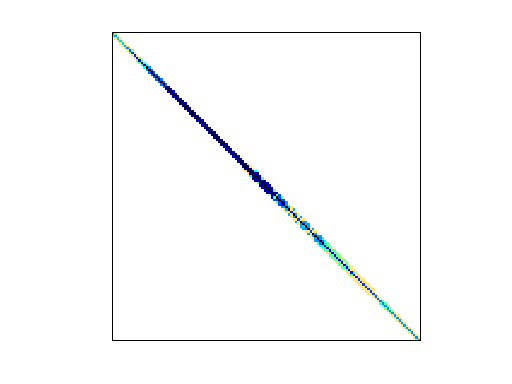
\includegraphics[width=1\textwidth]{figs/Flan_1565.png}
		\captionof{figure}{Flan-1565}
		\label{fig:Flan-1565}
	\end{minipage}
\end{table}

%######################################################################%
%||                                                                  %||
%||                                                                  %||
%||                            NEW MATRIX                            %||
%||                                                                  %||
%||                                                                  %||
%######################################################################%

\subsection{StocF-1465}
\begin{table}[h!]
	\begin{minipage}{0.5\linewidth}
		\caption{StocF-1465 Information}
		\label{table:StocF-1465}
		\centering
        \begin{tabular}{ll}
\midrule
                       Name &                           StocF-1465 \\
                      Group &                                Janna \\
                  Matrix ID &                                 2547 \\
                   Num Rows &                              1465137 \\
                   Num Cols &                              1465137 \\
                   Nonzeros &                             21005389 \\
            Pattern Entries &                             21005389 \\
                       Kind & CFDP \\
                  Symmetric &                                  Yes \\
                       Date &                                 2011 \\
                     Author &               C. Janna, M. Ferronato \\
                     Editor &                             T. Davis \\
            Structural Rank &                              1465137 \\
       Structural Rank Full &                                 true \\
          Num Dmperm Blocks &                                29105 \\
Strongly Connect Components &                                29105 \\
         Num Explicit Zeros &                                    0 \\
           Pattern Symmetry &                                 100\% \\
           Numeric Symmetry &                                 100\% \\
         Cholesky Candidate &                                  yes \\
          Positive Definite &                                  yes \\
                       Type &                                 real \\
\bottomrule
\end{tabular}

	\end{minipage}\hfill
	\begin{minipage}{0.45\linewidth}
		\centering
		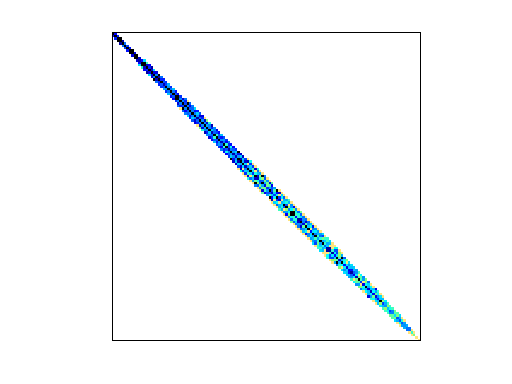
\includegraphics[width=1\textwidth]{figs/StocF-1465.png}
		\captionof{figure}{StocF-1465}
		\label{fig:StocF-1465}
	\end{minipage}
\end{table}


%######################################################################%
%||                                                                  %||
%||                                                                  %||
%||                            NEW MATRIX                            %||
%||                                                                  %||
%||                                                                  %||
%######################################################################%

\subsection{cfd2}
\begin{table}[h!]
	\begin{minipage}{0.5\linewidth}
		\caption{cfd2 Information}
		\label{table:cfd2}
		\centering
        \begin{tabular}{ll}
\midrule
                       Name &                                 cfd2 \\
                      Group &                             Rothberg \\
                  Matrix ID &                                  805 \\
                   Num Rows &                               123440 \\
                   Num Cols &                               123440 \\
                   Nonzeros &                              3085406 \\
            Pattern Entries &                              3087898 \\
                       Kind & CFDP \\
                  Symmetric &                                  Yes \\
                       Date &                                 1997 \\
                     Author &                          E. Rothberg \\
                     Editor &                             T. Davis \\
            Structural Rank &                               123440 \\
       Structural Rank Full &                                 true \\
          Num Dmperm Blocks &                                    1 \\
Strongly Connect Components &                                    1 \\
         Num Explicit Zeros &                                 2492 \\
           Pattern Symmetry &                                 100\% \\
           Numeric Symmetry &                                 100\% \\
         Cholesky Candidate &                                  yes \\
          Positive Definite &                                  yes \\
                       Type &                                 real \\
\bottomrule
\end{tabular}

	\end{minipage}\hfill
	\begin{minipage}{0.45\linewidth}
		\centering
		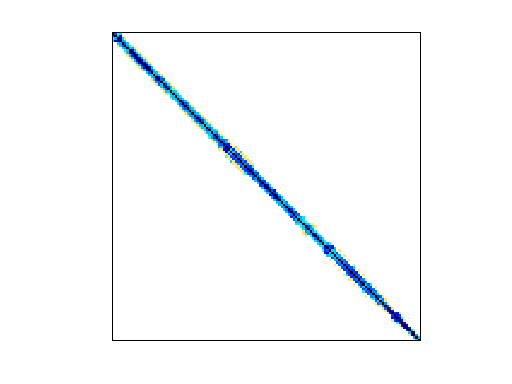
\includegraphics[width=1\textwidth]{figs/cfd2.png}
		\captionof{figure}{cfd2}
		\label{fig:cfd2}
	\end{minipage}
\end{table}


%######################################################################%
%||                                                                  %||
%||                                                                  %||
%||                            NEW MATRIX                            %||
%||                                                                  %||
%||                                                                  %||
%######################################################################%
\subsection{cfd1}
\begin{table}[h!]
	\begin{minipage}{0.5\linewidth}
		\caption{cdf1 Information}
		\label{table:cdf1}
		\centering
        \begin{tabular}{ll}
\midrule
                       Name &                                 cfd1 \\
                      Group &                             Rothberg \\
                  Matrix ID &                                  804 \\
                   Num Rows &                                70656 \\
                   Num Cols &                                70656 \\
                   Nonzeros &                              1825580 \\
            Pattern Entries &                              1828364 \\
                       Kind & CFDP \\
                  Symmetric &                                  Yes \\
                       Date &                                 1997 \\
                     Author &                          E. Rothberg \\
                     Editor &                             T. Davis \\
            Structural Rank &                                70656 \\
       Structural Rank Full &                                 true \\
          Num Dmperm Blocks &                                    1 \\
Strongly Connect Components &                                    1 \\
         Num Explicit Zeros &                                 2784 \\
           Pattern Symmetry &                                 100\% \\
           Numeric Symmetry &                                 100\% \\
         Cholesky Candidate &                                  yes \\
          Positive Definite &                                  yes \\
                       Type &                                 real \\
\bottomrule
\end{tabular}

	\end{minipage}\hfill
	\begin{minipage}{0.45\linewidth}
		\centering
		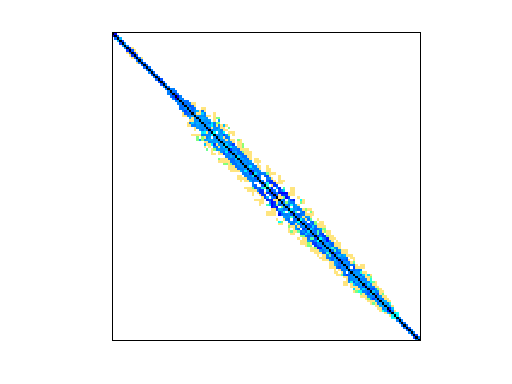
\includegraphics[width=1\textwidth]{figs/cfd1.png}
		\captionof{figure}{cdf1}
		\label{fig:cdf1}
	\end{minipage}
\end{table}



%######################################################################%
%||                                                                  %||
%||                                                                  %||
%||                            NEW MATRIX                            %||
%||                                                                  %||
%||                                                                  %||
%######################################################################%
\subsection{G3-circuit}
\begin{table}[h!]
	\begin{minipage}{0.5\linewidth}
		\caption{G3-circuit Information}
		\label{table:cdf1}
		\centering
        \begin{tabular}{ll}
\midrule
                       Name &                 G3\_circuit \\
                      Group &                        AMD \\
                  Matrix ID &                       1421 \\
                   Num Rows &                    1585478 \\
                   Num Cols &                    1585478 \\
                   Nonzeros &                    7660826 \\
            Pattern Entries &                    7660826 \\
                       Kind & Circuit Simulation Problem \\
                  Symmetric &                        Yes \\
                       Date &                       2006 \\
                     Author &                 U. Okuyucu \\
                     Editor &                   T. Davis \\
            Structural Rank &                    1585478 \\
       Structural Rank Full &                       true \\
          Num Dmperm Blocks &                          1 \\
Strongly Connect Components &                          1 \\
         Num Explicit Zeros &                          0 \\
           Pattern Symmetry &                       100\% \\
           Numeric Symmetry &                       100\% \\
         Cholesky Candidate &                        yes \\
          Positive Definite &                        yes \\
                       Type &                       real \\
\bottomrule
\end{tabular}

	\end{minipage}\hfill
	\begin{minipage}{0.45\linewidth}
		\centering
		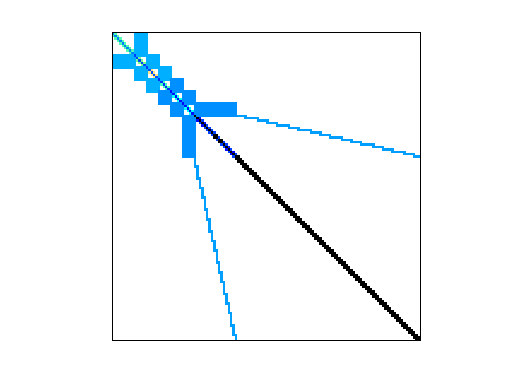
\includegraphics[width=1\textwidth]{figs/G3_circuit.png}
		\captionof{figure}{G3-circuit}
		\label{fig:G3-circuit}
	\end{minipage}
\end{table}



%######################################################################%
%||                                                                  %||
%||                                                                  %||
%||                            NEW MATRIX                            %||
%||                                                                  %||
%||                                                                  %||
%######################################################################%
\subsection{Parabolic Fem}
\begin{table}[h!]
	\begin{minipage}{0.5\linewidth}
		\caption{Parabolic Fem Information}
		\label{table:Parabolic Fem}
		\centering
        \begin{tabular}{ll}
\midrule
                       Name &                        parabolic\_fem \\
                      Group &                             Wissgott \\
                  Matrix ID &                                 1853 \\
                   Num Rows &                               525825 \\
                   Num Cols &                               525825 \\
                   Nonzeros &                              3674625 \\
            Pattern Entries &                              3674625 \\
                       Kind & CFDP \\
                  Symmetric &                                  Yes \\
                       Date &                                 2007 \\
                     Author &                          P. Wissgott \\
                     Editor &                             T. Davis \\
            Structural Rank &                               525825 \\
       Structural Rank Full &                                 true \\
          Num Dmperm Blocks &                                    1 \\
Strongly Connect Components &                                    1 \\
         Num Explicit Zeros &                                    0 \\
           Pattern Symmetry &                                 100\% \\
           Numeric Symmetry &                                 100\% \\
         Cholesky Candidate &                                  yes \\
          Positive Definite &                                  yes \\
                       Type &                                 real \\
\bottomrule
\end{tabular}

	\end{minipage}\hfill
	\begin{minipage}{0.45\linewidth}
		\centering
		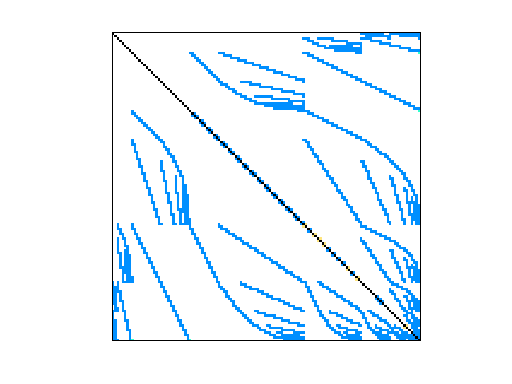
\includegraphics[width=1\textwidth]{figs/parabolic_fem.png}
		\captionof{figure}{Parabolic Fem}
		\label{fig:Parabolic Fem}
	\end{minipage}
\end{table}



%######################################################################%
%||                                                                  %||
%||                                                                  %||
%||                            NEW MATRIX                            %||
%||                                                                  %||
%||                                                                  %||
%######################################################################%
\subsection{apache2}
\begin{table}[h!]
	\begin{minipage}{0.5\linewidth}
		\caption{apache2 Information}
		\label{table:apache2}
		\centering
        \begin{tabular}{ll}
\midrule
                       Name &                   apache2 \\
                      Group &                 GHS\_psdef \\
                  Matrix ID &                      1423 \\
                   Num Rows &                    715176 \\
                   Num Cols &                    715176 \\
                   Nonzeros &                   4817870 \\
            Pattern Entries &                   4817870 \\
                       Kind &        Structural Problem \\
                  Symmetric &                       Yes \\
                       Date &                      2006 \\
                     Author &                       NaN \\
                     Editor & N. Gould, Y. Hu, J. Scott \\
            Structural Rank &                    715176 \\
       Structural Rank Full &                      true \\
          Num Dmperm Blocks &                         1 \\
Strongly Connect Components &                         1 \\
         Num Explicit Zeros &                         0 \\
           Pattern Symmetry &                      100\% \\
           Numeric Symmetry &                      100\% \\
         Cholesky Candidate &                       yes \\
          Positive Definite &                       yes \\
                       Type &                      real \\
\bottomrule
\end{tabular}

	\end{minipage}\hfill
	\begin{minipage}{0.45\linewidth}
		\centering
		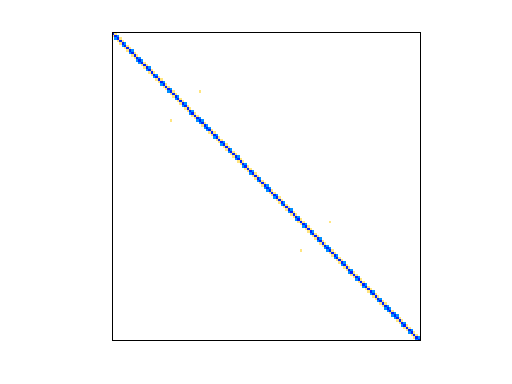
\includegraphics[width=1\textwidth]{figs/apache2.png}
		\captionof{figure}{apache2}
		\label{fig:apache2}
	\end{minipage}
\end{table}



%######################################################################%
%||                                                                  %||
%||                                                                  %||
%||                            NEW MATRIX                            %||
%||                                                                  %||
%||                                                                  %||
%######################################################################%
\subsection{shallow water1}
\begin{table}[h!]
	\begin{minipage}{0.5\linewidth}
		\caption{shallow water1 Information}
		\label{table:shallow water1}
		\centering
        \begin{tabular}{ll}
\midrule
                       Name &                       shallow\_water1 \\
                      Group &                            MaxPlanck \\
                  Matrix ID &                                 2261 \\
                   Num Rows &                                81920 \\
                   Num Cols &                                81920 \\
                   Nonzeros &                               327680 \\
            Pattern Entries &                               327680 \\
                       Kind & CFDP \\
                  Symmetric &                                  Yes \\
                       Date &                                 2009 \\
                     Author &               K. Leppkes, U. Naumann \\
                     Editor &                             T. Davis \\
            Structural Rank &                                81920 \\
       Structural Rank Full &                                 true \\
          Num Dmperm Blocks &                                    1 \\
Strongly Connect Components &                                    1 \\
         Num Explicit Zeros &                                    0 \\
           Pattern Symmetry &                                 100\% \\
           Numeric Symmetry &                                 100\% \\
         Cholesky Candidate &                                  yes \\
          Positive Definite &                                  yes \\
                       Type &                                 real \\
\bottomrule
\end{tabular}

	\end{minipage}\hfill
	\begin{minipage}{0.45\linewidth}
		\centering
		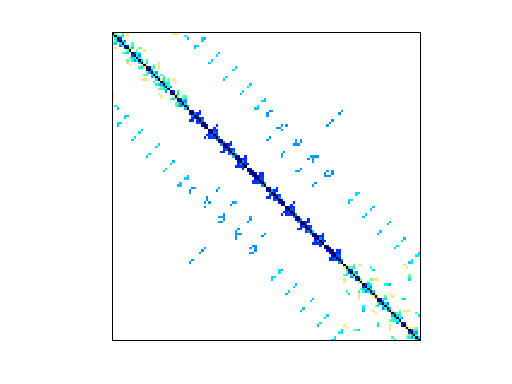
\includegraphics[width=1\textwidth]{figs/shallow_water1.png}
		\captionof{figure}{shallow water1}
		\label{fig:shallow water1}
	\end{minipage}
\end{table}




%######################################################################%
%||                                                                  %||
%||                                                                  %||
%||                            NEW MATRIX                            %||
%||                                                                  %||
%||                                                                  %||
%######################################################################%
\subsection{ex15}
\begin{table}[h!]
	\begin{minipage}{0.5\linewidth}
		\caption{ex15 Information}
		\label{table:ex15}
		\centering
        \begin{tabular}{ll}
\midrule
                       Name &                                 ex15 \\
                      Group &                                FIDAP \\
                  Matrix ID &                                  413 \\
                   Num Rows &                                 6867 \\
                   Num Cols &                                 6867 \\
                   Nonzeros &                                98671 \\
            Pattern Entries &                                98671 \\
                       Kind & CFDP \\
                  Symmetric &                                  Yes \\
                       Date &                                 1994 \\
                     Author &                   A. Baggag, Y. Saad \\
                     Editor &                   A. Baggag, Y. Saad \\
            Structural Rank &                                 6867 \\
       Structural Rank Full &                                 true \\
          Num Dmperm Blocks &                                    2 \\
Strongly Connect Components &                                    2 \\
         Num Explicit Zeros &                                    0 \\
           Pattern Symmetry &                                 100\% \\
           Numeric Symmetry &                                 100\% \\
         Cholesky Candidate &                                  yes \\
          Positive Definite &                                  yes \\
                       Type &                                 real \\
\bottomrule
\end{tabular}

	\end{minipage}\hfill
	\begin{minipage}{0.45\linewidth}
		\centering
		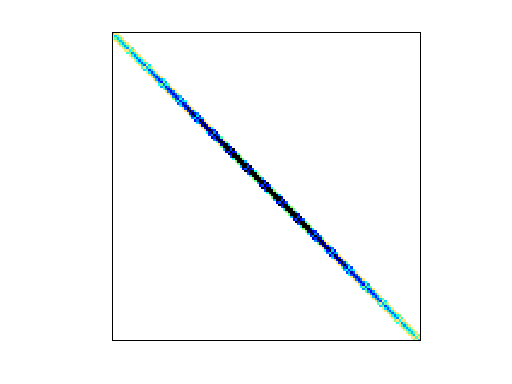
\includegraphics[width=1\textwidth]{figs/ex15.png}
		\captionof{figure}{ex15}
		\label{fig:ex15}
	\end{minipage}
\end{table}

\section{Risulti Sperimentali}
\subsection{Confronto OS: Windows e Linux}
\subsection{Confronto Linguaggi: Python e Matlab}
\subsection{Altri Risultati Sperimentali}
\paragraph{Errore relativo e Condizionamento delle Matrici}
\paragraph{}
\section{Conclusioni}





% BIBLIOGRAPHY
\bibliographystyle{unsrtnat}
\bibliography{references}  %%% Uncomment this line and comment out the ``thebibliography'' section below to use the external .bib file (using bibtex) .


%%% Uncomment this section and comment out the \bibliography{references} line above to use inline references.
% \begin{thebibliography}{1}

% 	\bibitem{kour2014real}
% 	George Kour and Raid Saabne.
% 	\newblock Real-time segmentation of on-line handwritten arabic script.
% 	\newblock In {\em Frontiers in Handwriting Recognition (ICFHR), 2014 14th
% 			International Conference on}, pages 417--422. IEEE, 2014.

% 	\bibitem{kour2014fast}
% 	George Kour and Raid Saabne.
% 	\newblock Fast classification of handwritten on-line arabic characters.
% 	\newblock In {\em Soft Computing and Pattern Recognition (SoCPaR), 2014 6th
% 			International Conference of}, pages 312--318. IEEE, 2014.

% 	\bibitem{hadash2018estimate}
% 	Guy Hadash, Einat Kermany, Boaz Carmeli, Ofer Lavi, George Kour, and Alon
% 	Jacovi.
% 	\newblock Estimate and replace: A novel approach to integrating deep neural
% 	networks with existing applications.
% 	\newblock {\em arXiv preprint arXiv:1804.09028}, 2018.

% \end{thebibliography}


\end{document}
